% vim: set tw=78 sts=2 sw=2 ts=8 aw et ai:

\begin{figure}[htb]
  \begin{center}
    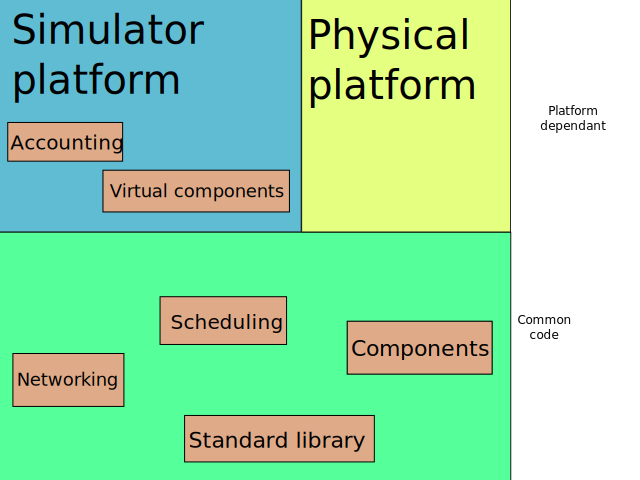
\includegraphics[scale=0.75]{img/bigarch.pdf}
    \caption{Hive simulator Architecture}
  \end{center}
\end{figure}


\subsection{Controlling the simulator}

The simulator is controlled through simple commands on a TCP socket. For
example to load a test plugin, start it, stop it and then unload it we would
do:
\begin{lstlisting}
$ nc 127.0.0.1 54321
load test
1
start 1
stop 1
unload 1
\end{lstlisting}
If the library test.so is not found in LD_LIBRARY_PATH an error will be
thrown.
